\documentclass[../root]{subfiles}
\graphicspath{{_images/}{../_images/}}

\begin{document}

    \chapter{Integrating Immigrants: The Impact of Restructuring Active Labor Market Program}

    \begin{shortsummary}
        \begin{itemize}
            \item \authoryear{Sarvimaki2016} %正しいキーワードに修正する
            \item \RQ{Does restructuring active labor market program for unemployment in Finland efficiently work?}
            \item \answer{Estimating by RDD.}
            \item \result{It increased compliers' cumulative earnings by 47\% and 13\% over 10 year follow-up period.  }
        \end{itemize}
    \end{shortsummary}

    \section{Introduction}

    This paper examine the active labor market program (ALMP) for disadvantaged immigrants can be remarkably efficient. \\
    
    \begin{figure}[h]
        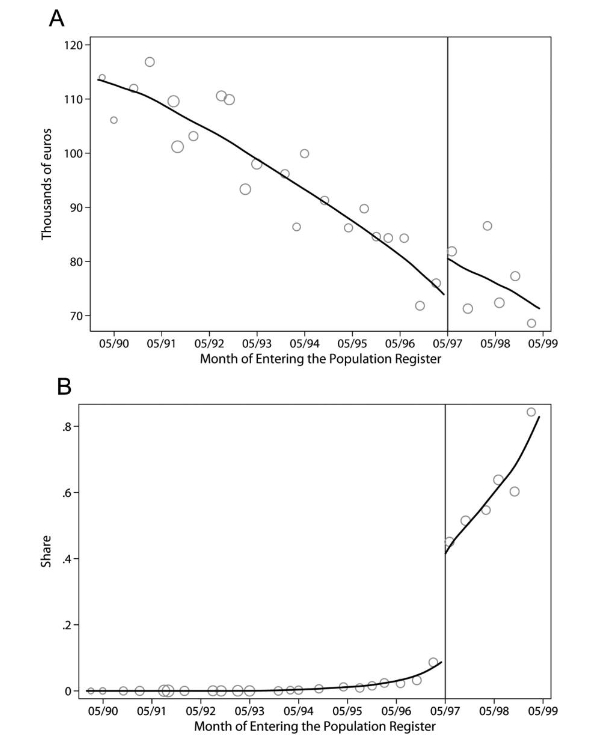
\includegraphics[width=12cm]{0703sugiyama/Figure1.png}
    \end{figure}
    
    Figure 1 show the discontinuous relationship of month of entering the population register, and earnings and share of receiving an integration plan.  \\  
    This reform force on 1999, May 1. But, it affected only those immigration who arrived after May 1, 1997. \\
    {\bf The ALMP impact on immigration }
    \begin{itemize}
        \item The participating immigration earned roughly 7000 euro more during the 2000s.
        \item They were 35 \% more likely to get an integration plan.
    \end{itemize}
        Together the discontinuities suggest a local average treatment effect of 21,000 euro and 13 \% decrease in cumulative social benefits. \\
        
        This paper show that there are no discontinuities in the number of immigrants arriving at the cut off and that their conclusions are not sensitive to the choice of bandwidth. \\
    
    {\bf Contribution} 
    \begin{itemize}
        \item Typically, literature of studying about ALMP estimated the impact on native, but, this paper estimate the impact of ALMP on immigrants.
        \item This paper show language training contribute the labor market integration. Improving language skills is often hypothesis to play an important role, but it is difficult because of measurement error and endogeneity problems . 
    \end{itemize}
    
    \section{Treatment}
    {\bf Background} \\
    This paper estimate the impact of as part of the Act of the Integration of Immigrants and Reception of Asylum Seekers force on May 1, 1999. \\
    The poor labor market performance arrivals in 1990s and their employment rate very low.  \\
    Low average employment rates led to high average social benefits received by immigrant households. \\
    {\bf Integration} \\
    The main change that employment offices had to start individualized  integration plans for non working immigrants who had lived in Finland for less than 3 years.  \\
    The plants were prepared in a joint meeting with caseworkers and immigrants.The aim was to find a sequence of training and other measures that would be the must suitable for each immigrants given her or his skills and circumstance.  \\
    The "treatment" authors examine is best to understand as an increased focus on the circumstance of each immigrant during a time when the supply of suitable training was being increased. 
    
    
    \section{Empirical strategy}
    {\bf Identification} \\
    We can identify the local average treatment effect (LATE) under the standard monotonicity and continuity assumption.
    
    \begin{itemize}
        \item Monotonicity : No one became less likely to receive an integration plan if she or he entered the population register on May 1, 1997, rather than the day before.
        \item Continuity : Those entering the population  just before and after the cutoff data has similar potential outcomes.
    \end{itemize}
    
    {\bf Estimation} \\
    This paper estimate the impact using the regression discontinuity (RD) design. \\
    This paper use only immigration who entered the population register before May 1999 and triangle-sharped Kernel that put most weight on those arriving close to the cutoff. \\
    Authors use algorithm proposed by Imbens and Kalyanarman (2012) for choosing  optimal bandwidth. \\
    
    The reduced form as follow
    \begin{align*}
        y_i = \alpha +\beta {\bf1}[r_i \geq r_0] + \delta_0(r_i- r_0) + \delta_1 {\bf1}[r_i \geq r_0] (r_i- r_0) +X_i \theta + \epsilon_i, 
    \end{align*}
    where $y_i$ is outcome, ${\bf 1}[\cdot]$ is an indicator, $r_i$ is date of entering the population register, $r_0$ is May 1, 1997, $X_i$ is a vector of observed characteristic measured at the year of arrival, and $\epsilon_i$ is unobserved factors.  \\
    
    Similarly, authors estimate the first-stage as 
    \begin{align*}
        D_i = \mu + \gamma {\bf 1}[r_i \geq r_0] + \lambda_0(r_i - r_0)  +\lambda_1 {\bf 1}[r_i \geq r_0](r_i - r_0) +X_i \pi + v_i,
    \end{align*}
    where $D_i$ is an indicator for immigrant $i$ getting on integration plan. \\
    The parameter of interest are $\beta$ and $\gamma$, which measure the jump in the expected outcome. \\
    They correspond to the numerator and the denominator of a Wald estimator.
    The estimate for LATE is $\hat{\tau} =\hat{\beta}/\hat{\gamma} $, which can be estimated using standard weighted 2SLS.
     
     Authors estimate compliers' potential outcomes in the absence of an integration plan by using $y_i(1-D_i)$ as the dependent variable and $(1-D_i)$ as the treatment variable in 2SLS regression.
    \section{Data}
    {\bf Sources and Sample} \\
    This paper use Statistics Finland data. \\
    Authors access to 90 \% random sampling of immigrants who arrived between January 1990 and April 1999, and authors focus on those who were targeted by the policy. \\
    Observations are 16,615.\\
    
    {\bf Background Characteristics} \\
    Table 1 present immigrants' average background characteristics by the date of arrival.
    
    \begin{figure}[h]
        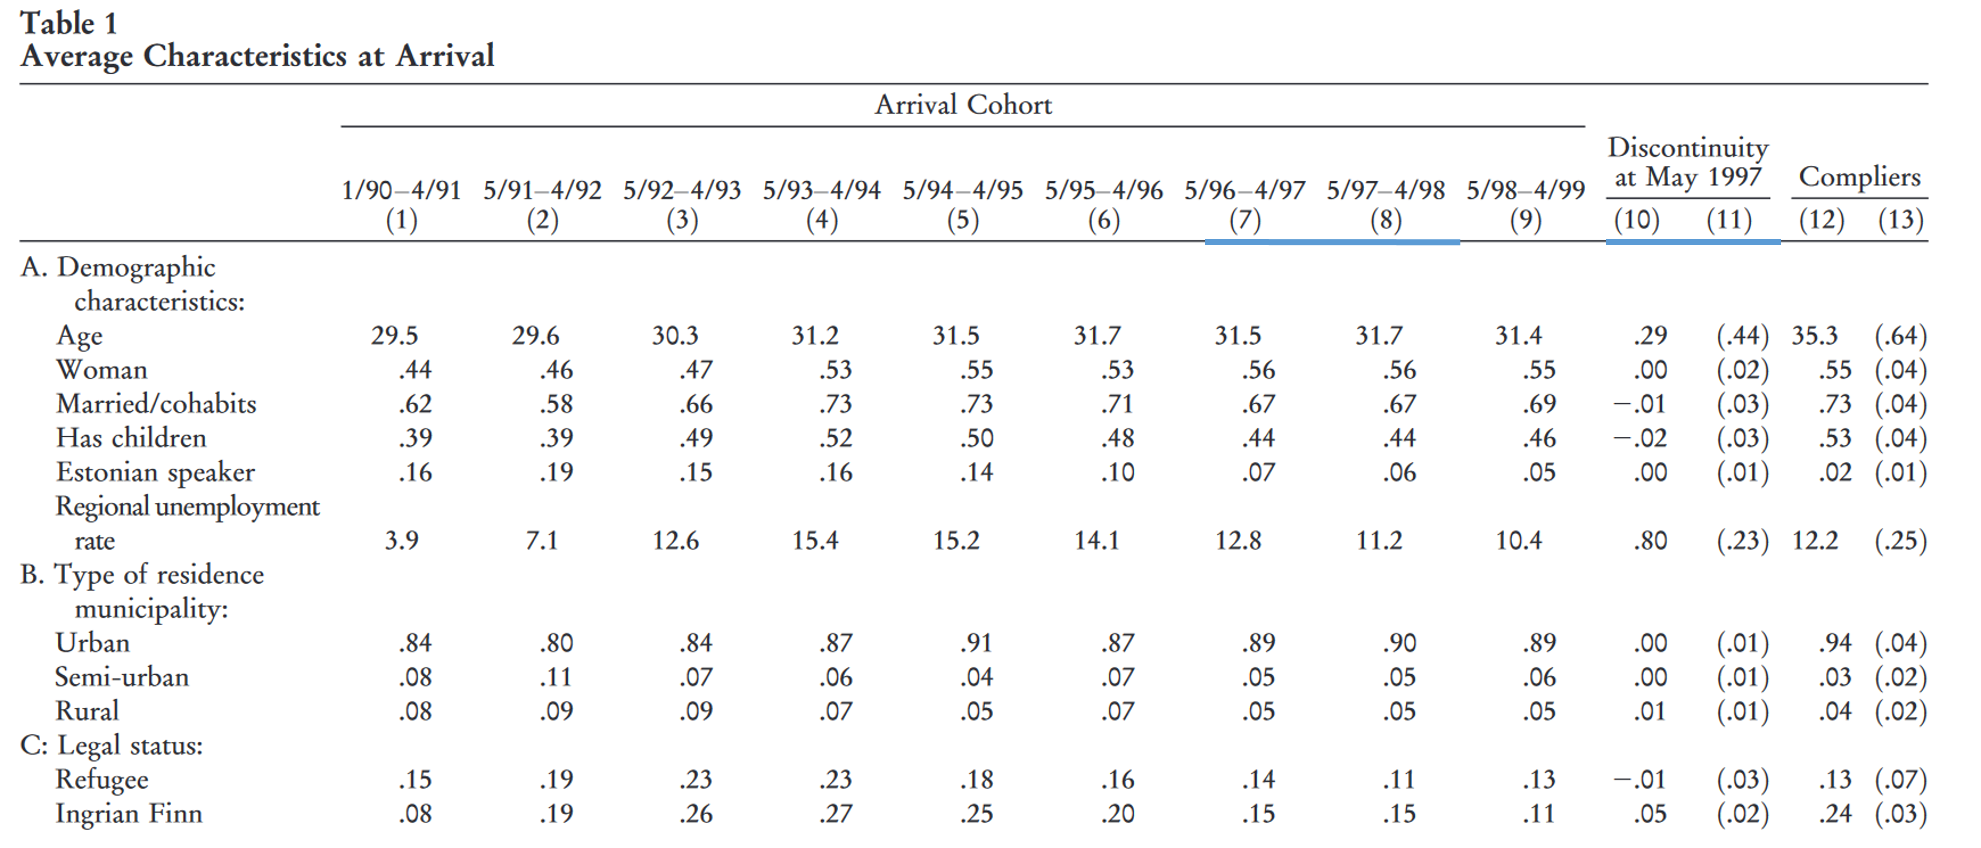
\includegraphics[width=14cm]{0703sugiyama/Table11.png}
    \end{figure}
    
    \begin{figure}[h]
        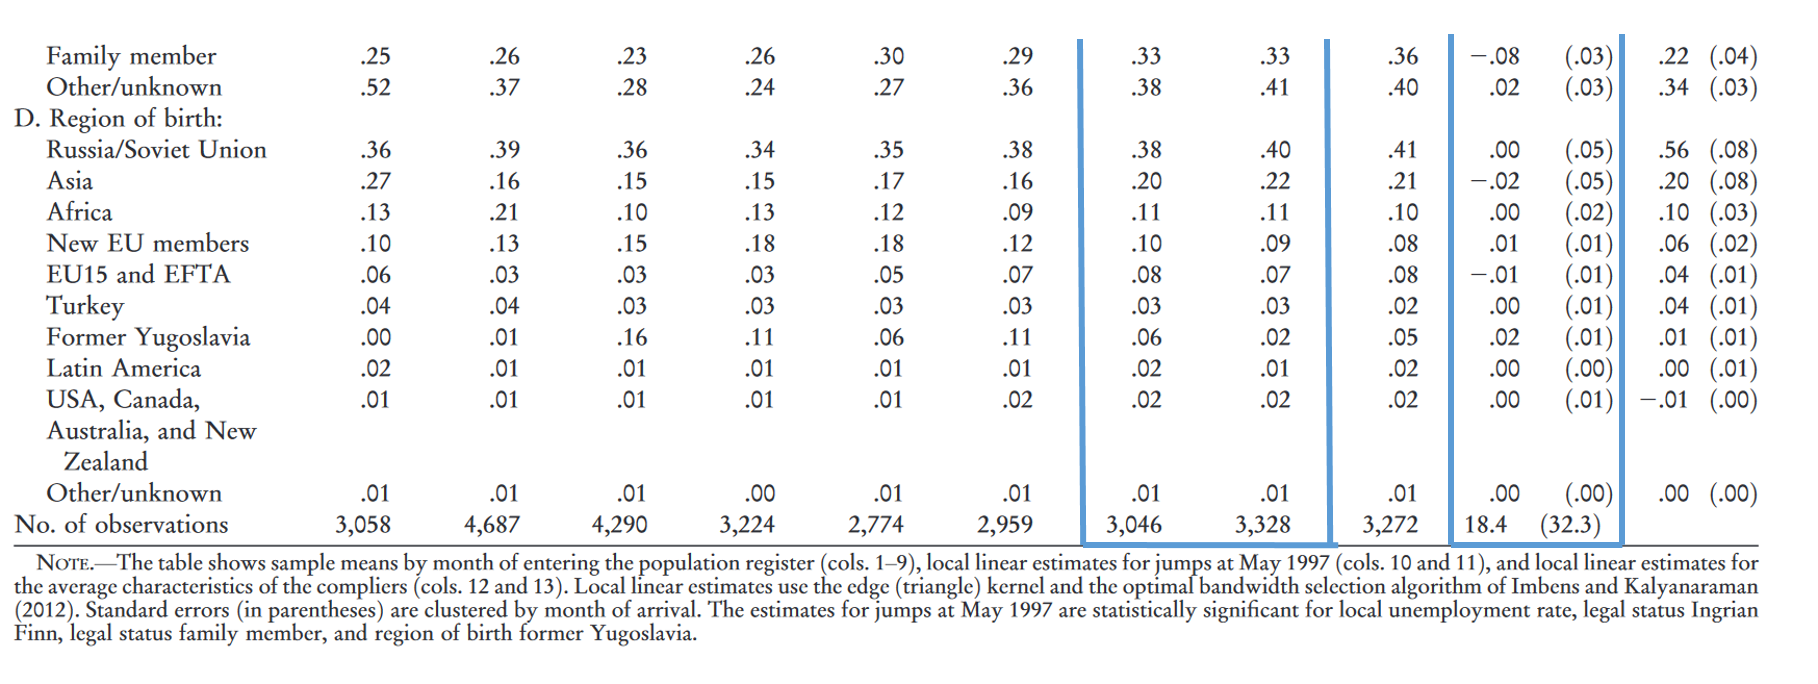
\includegraphics[width=14cm]{0703sugiyama/Table12.png}
    \end{figure}
    
    A casual comparison of column 7 and 8 suggest that immigrants arriving a year before and after the May 1997 cutoff were very similar.  \\
    
    Estimate reported in column 10, six are significant and the difference in back ground characters are small. \\
    Those who arrived in May 1997 had less favorable background characteristics than those arrived just before. \\
    
    {\bf Outcomes}
    
    Table 2 presents outcome variables.
    \begin{figure}[h]
        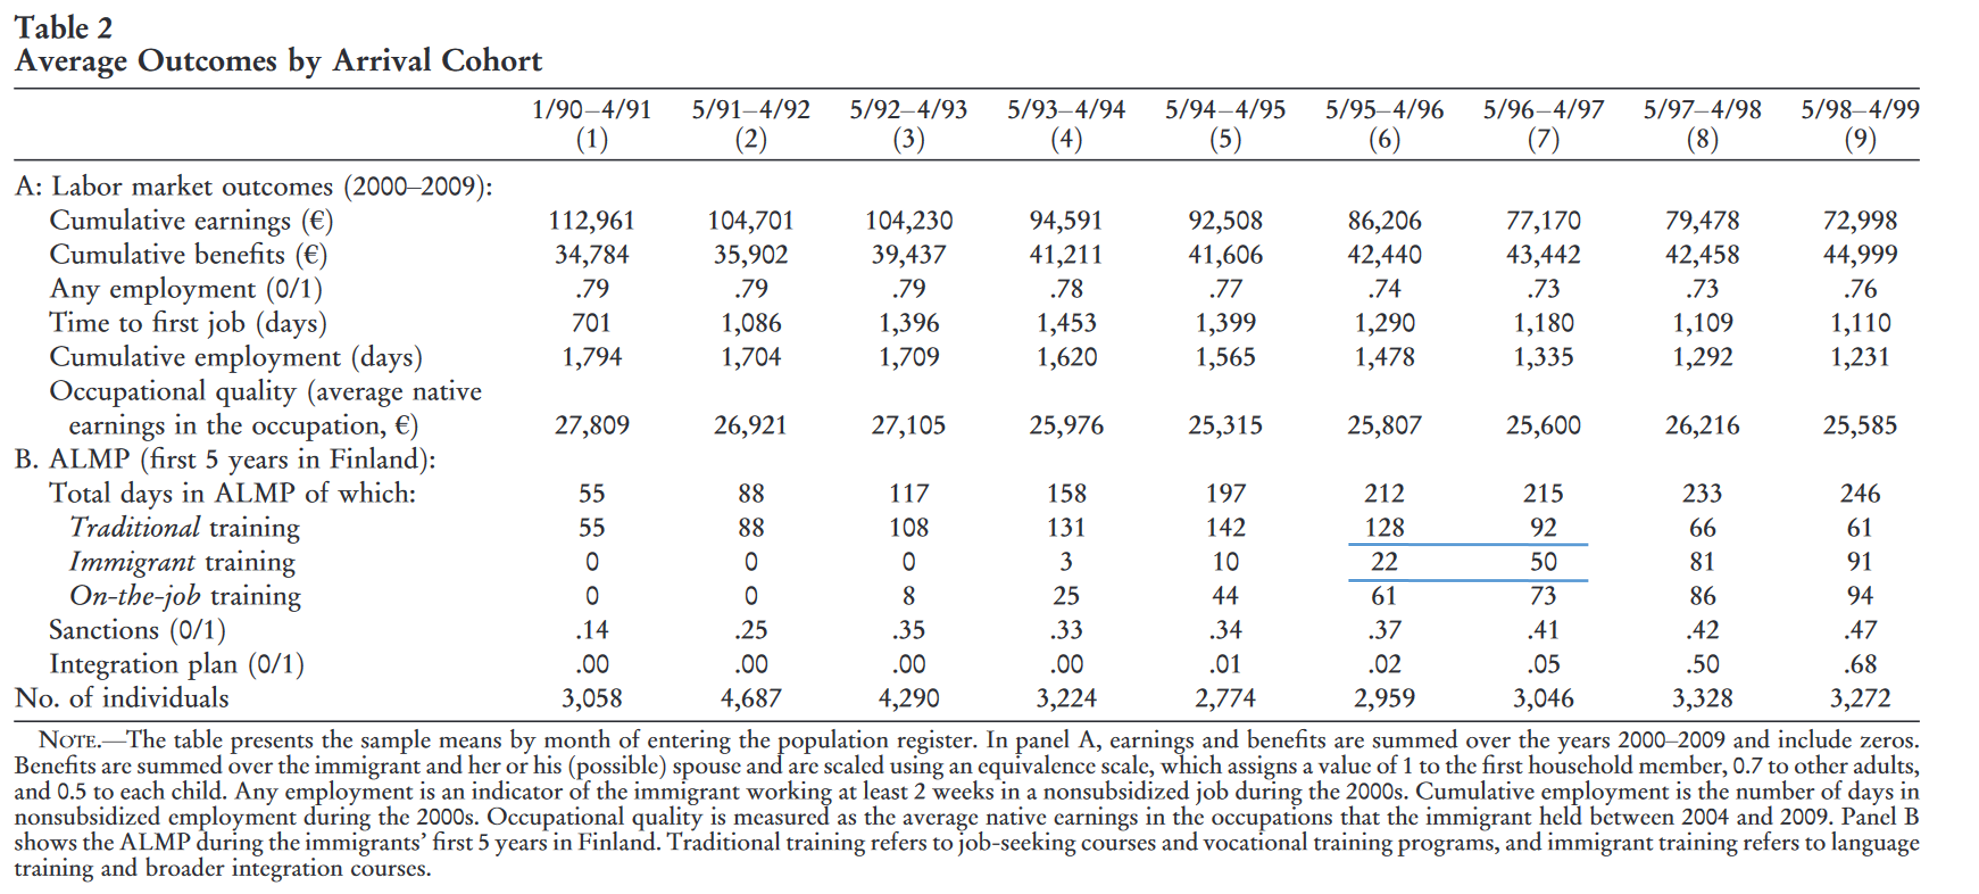
\includegraphics[width=14cm]{0703sugiyama/Table2.png}
    \end{figure}
    
    %Table 2 check later.
    Primary measure for economic performance is cumulative earnings over the period 2000-2009. \\
    Authors also examine a similar measure of household level social benefits. \\
    The bottom panel presents their measure of ALMP. \\
    \begin{itemize}
        \item Among the earlier cohorts, this growth is largely driven by an increasing "traditional training", such as job-seeking course and vocational training program.
        \item For the later cohorts, traditional program is replaced by language training and broader integration courses.
    \end{itemize}
    
    \section{Results}
    {\bf Earnings and benefits} \\
    Table 3 presents main results.
    
    \begin{figure}[h]
        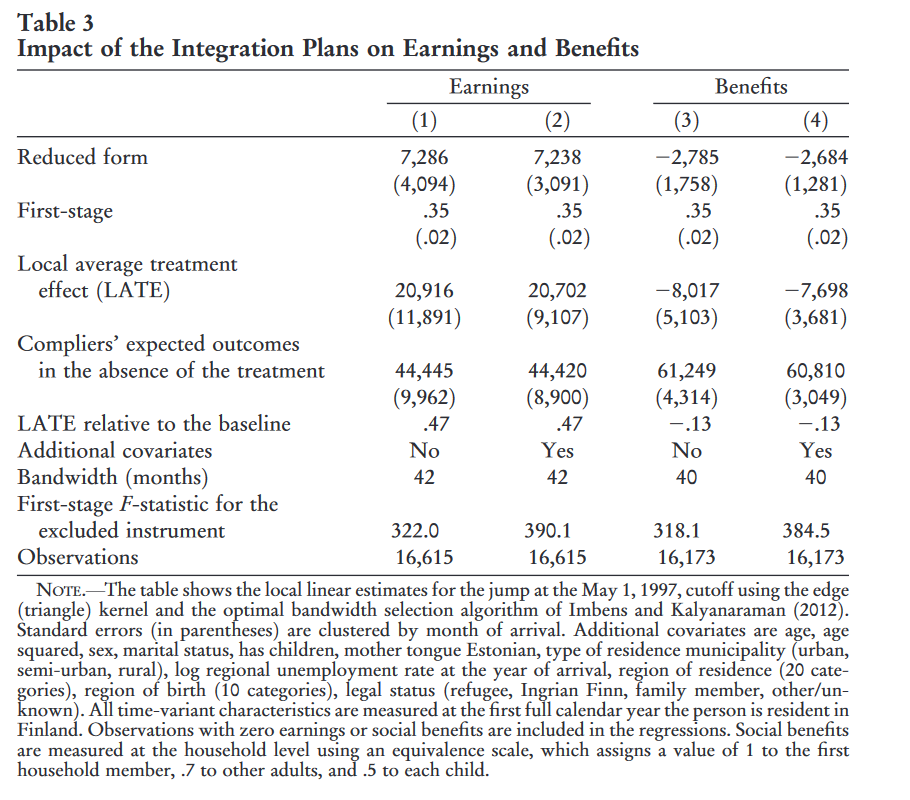
\includegraphics[width=12cm]{0703sugiyama/Table3.png}
    \end{figure}
    
    
    {\bf The effect to earnings } \\
    \begin{itemize}
        \item A LATE of a 20,961 euro  increase in earnings over decade.
        \item Expected outcome among complier if they had not received an integration plan is 44,445 in the 2000s and thus the LATE estimate correspond to 47\% increase in their earnings
        \item The results is not depend on whether authors take into account observable characteristics.  
    \end{itemize}
    
    
    {\bf The effect to social benefits}
    \begin{itemize}
        \item A 2,785 euro decline at May 1997 cutoff.
        \item A LATE of 8,01 corresponding to a 13\% decreasing in benefits.
    \end{itemize}
    Figure 2 represents benefits results graphically.
    
    \begin{figure}[h]
        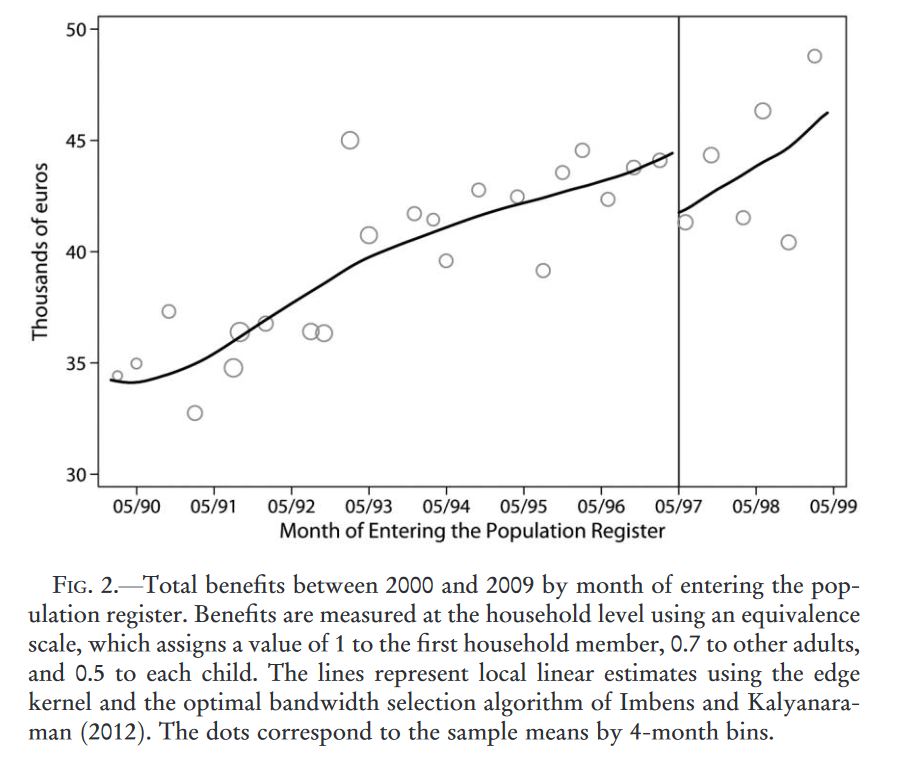
\includegraphics[width=12cm]{0703sugiyama/Figure2.png}
    \end{figure}
    
    {\bf Validity of research design} \\
    The reason why authors think these estimation as casual impact.
    \begin{itemize}
        \item Immigrants' observable characteristics evolve smoothly over the cutoff point.
        \item The research design passes the McCrary (2008) Density Test.(col 10 and 11 in the last raw of table 1)
        \item Authors reach similar conclusion regardless of the chosen bandwidth(figure 3).
    \end{itemize}
    
    \begin{figure}[h]
        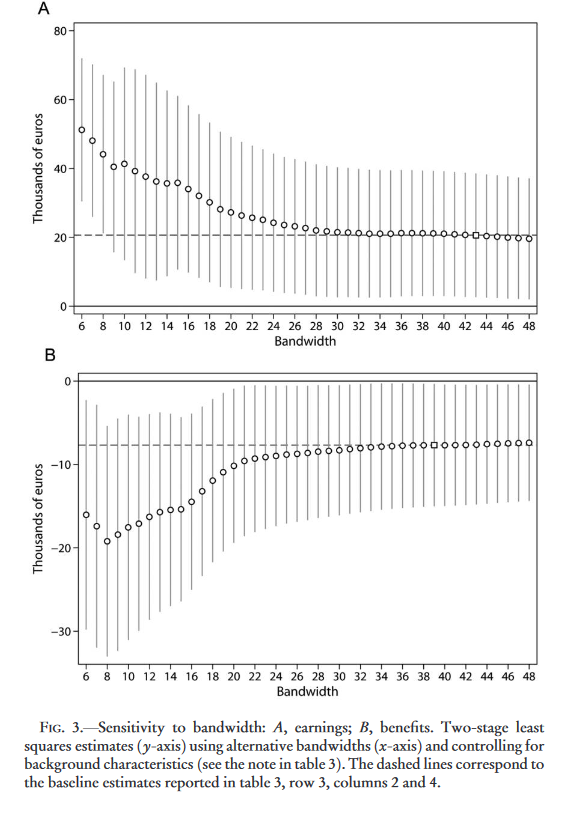
\includegraphics[width=12cm]{0703sugiyama/Figure3.png}
    \end{figure}
    
    Their baseline estimates can be regarded as conservative because shorter bandwidth results in much larger effects. \\
    
    Figure 4 presents the results of placebo cutoffs. Authors set the cutoff point at each month between May 1993 and May 1996. \\
    Of the 72  resulting estimates only three are larger absolute value than main estimates and thus baseline results appear robust.
    \begin{figure}[h]
        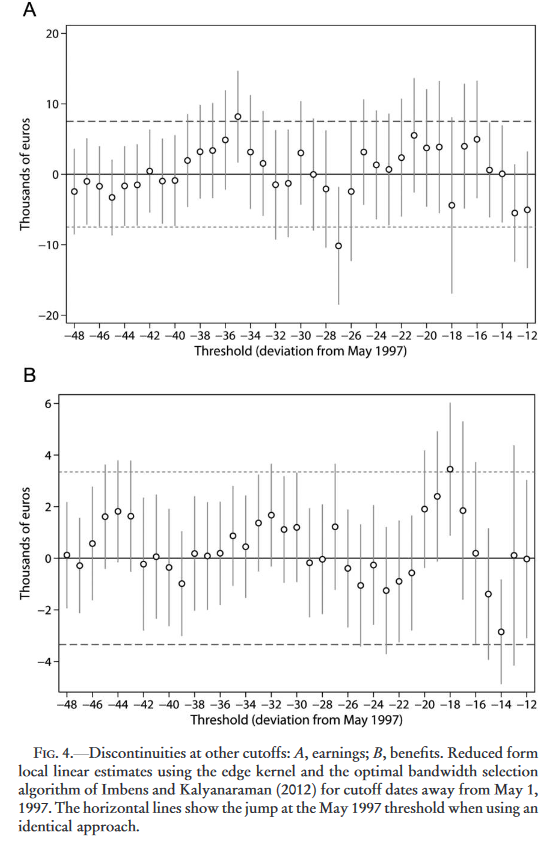
\includegraphics[width=12cm]{0703sugiyama/Figure4.png}
    \end{figure}
    
    {\bf Employment and Occupation} \\
    Figure 5 and table 4 examine whether integration plans affect earnings through hours, wages, or both. \\
    
    No evidence of impact on the likelihood of any employment, the time to the first job, or the total days employed. However, it is important to bear in mind that authors cannot distinguish between part-time and full-time work. \\
    The integration plans seem to have helped immigrants to enter occupations associated 6\% - 8\% higher earnings.
    
    
    
    \begin{figure}[h]
        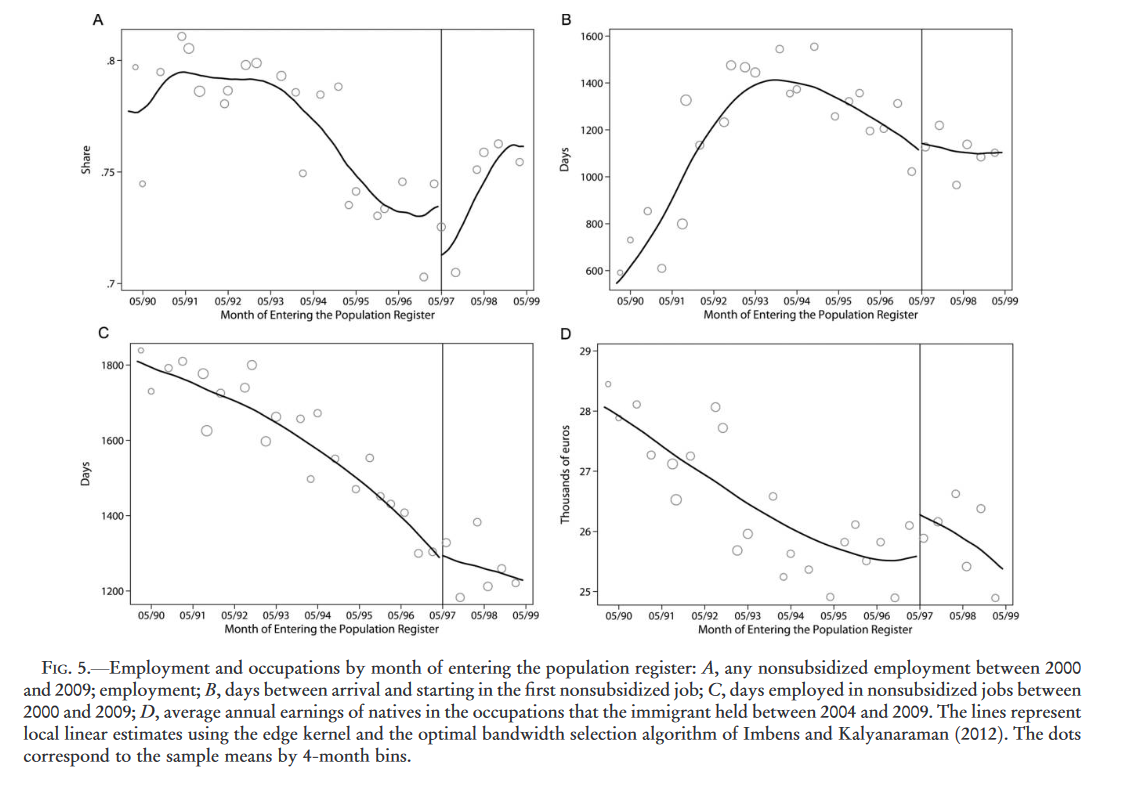
\includegraphics[width=12cm]{0703sugiyama/Figure5.png}
    \end{figure}
    
    \begin{figure}[h]
        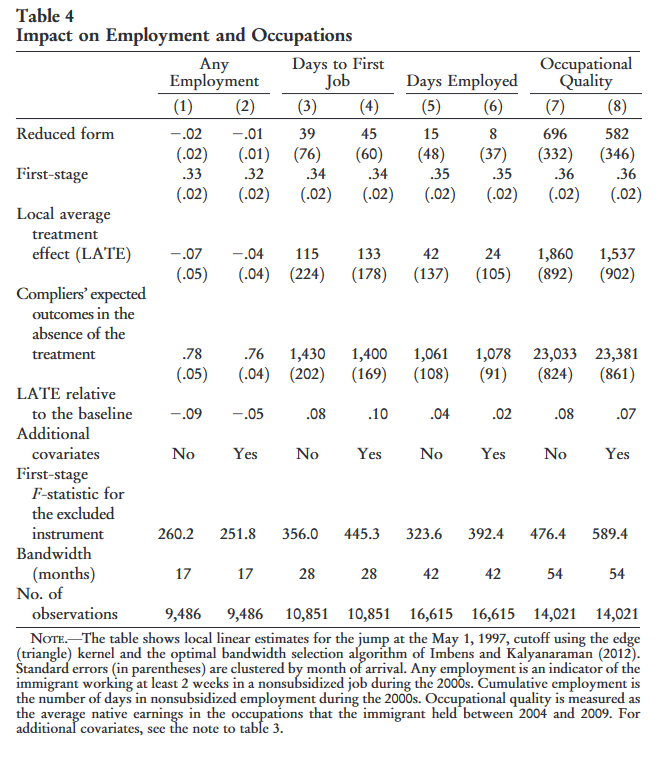
\includegraphics[width=12cm]{0703sugiyama/Table4.png}
    \end{figure}
    
    {\bf Training and Sanctions} \\
    Figure 6 and 7 and table 5 examine how integration plan affected the amount and type of ALMP. \\
    These plans did not lead to more training.  \\
    Instead, integration plans appear to have changed the content of training. Figure 7 shows that "immigrants training"  increase 10 \% due to receiving an integration plan. \\
    Correspondingly, "traditional training" started to decline already among cohorts who arrived in Finland before the cutoff, but authors find a negative LATE of 30 days, or 7\%, at the May 1997 cutoff. 
  \begin{figure}[h]
        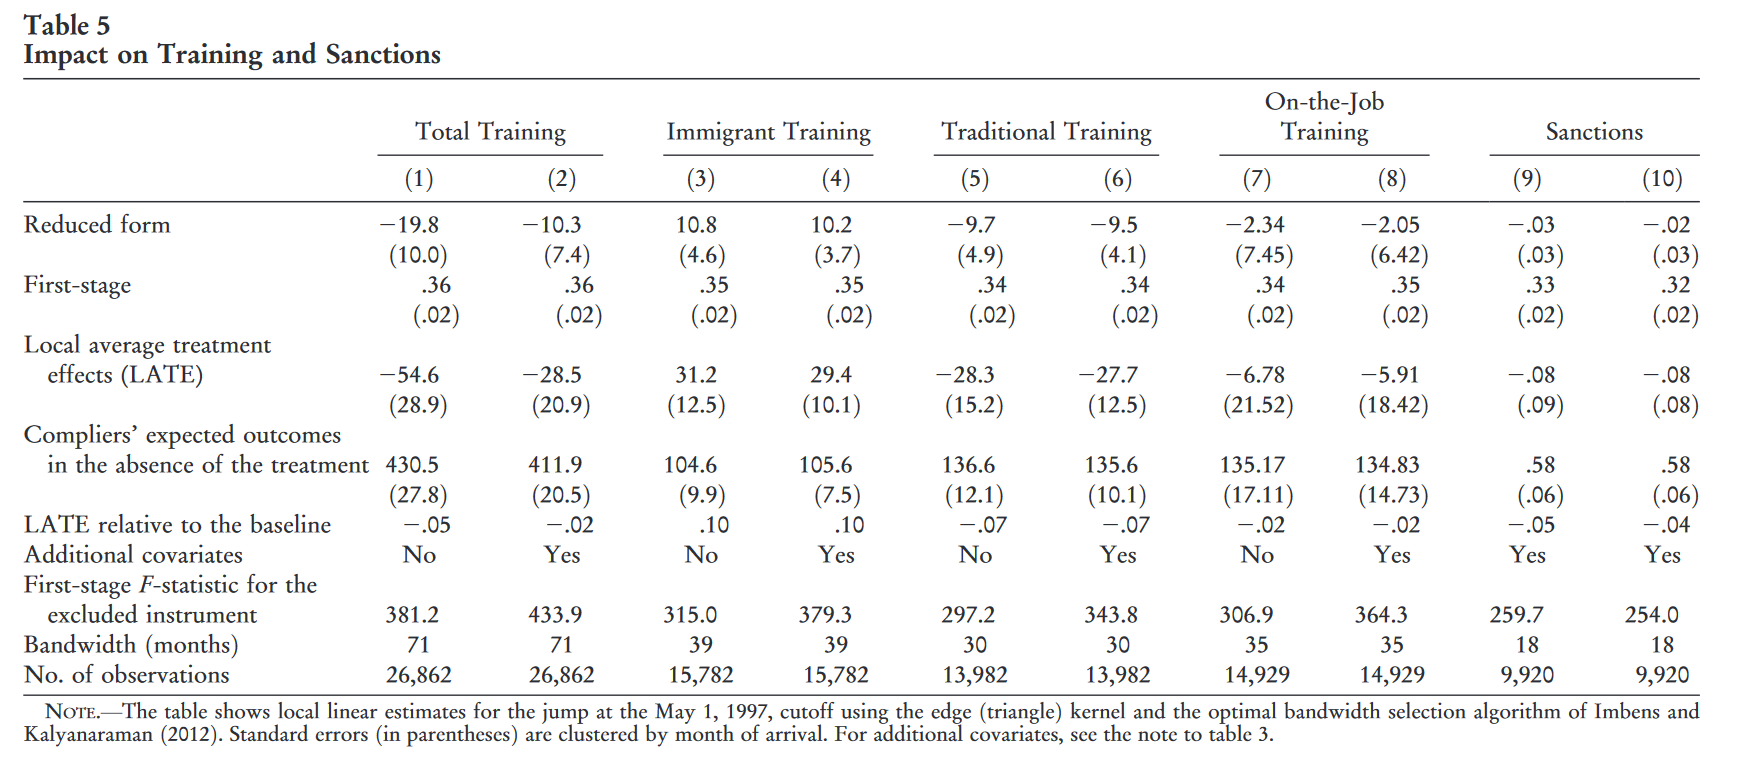
\includegraphics[width=15cm]{0703sugiyama/Table5.png}
    \end{figure}
    \begin{figure}[h]
        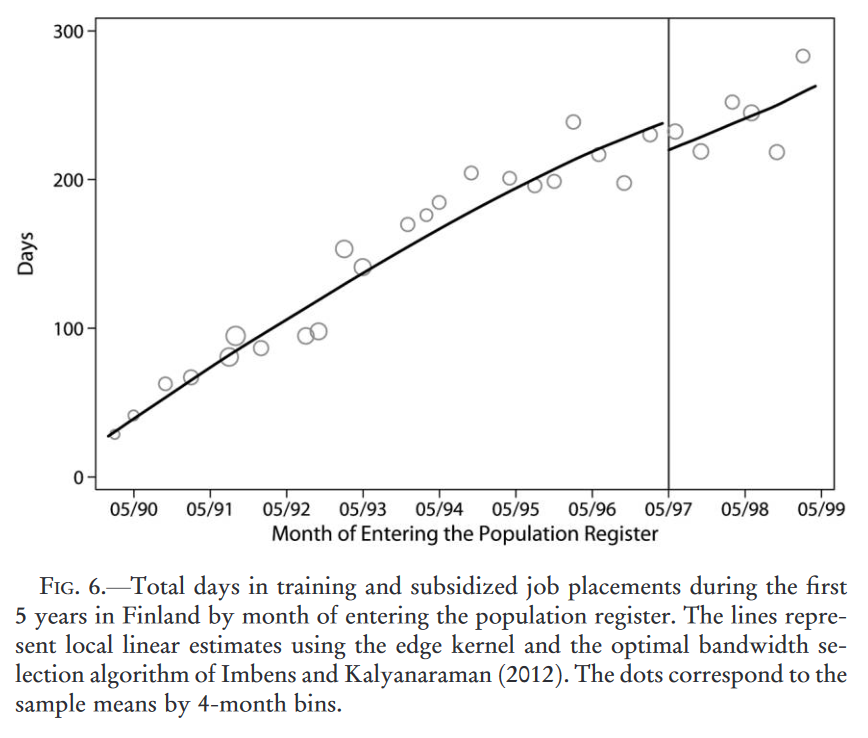
\includegraphics[width=12cm]{0703sugiyama/Figure6.png}
    \end{figure}
    \begin{figure}[h]
        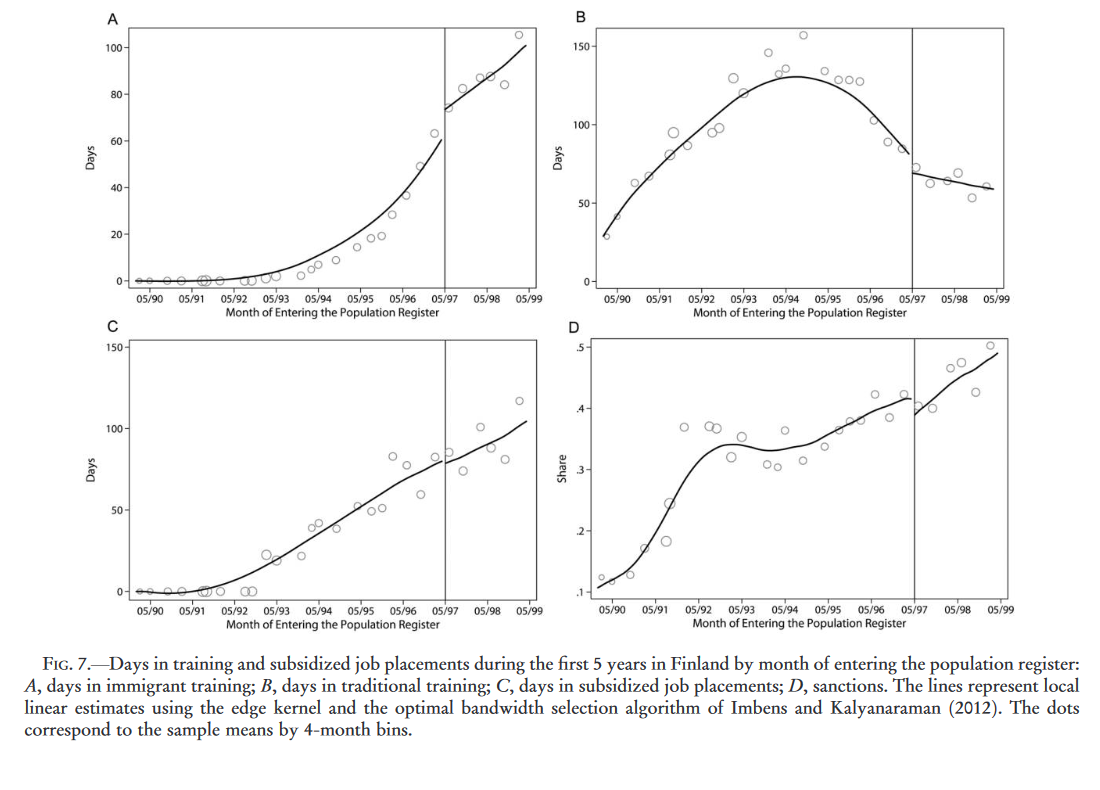
\includegraphics[width=15cm]{0703sugiyama/Figure7.png}
    \end{figure}
    While the share of immigrants facing sanctions increased over time, there is no statistically significant jump at the May 1997 cutoff. It is reason why the reform did not affect the rules governing the use of sanctions.
    
    {\bf Compliers} \\
    The estimation for potential outcomes whose immigrants arrived between May 1999 and April 2000 indicate that without integration plan, they would have earned only about 4,500 euro per year and collected more than 6,000 euro benefits per year during the 2000s. \\
    In comparison, Authors also estimate the potential outcomes and benefits among immigrants who entered between May and December 1997.  The results were 9,400 euro and 3,300 euro,respectively. \\
    From the table 1, compliers were a few years older than other immigrnts and less likely to speak Estonian as their mother tongue, to come from high-income countries, or to have arrived as a family size. 
    
    {\bf Costs and Benefits} \\
    The costs of the reform appear to be due to the Labor Administration and the time that caseworkers and interpreters spent in the preparation and monitoring of integration plans. \\
    A typical integration plan takes about 1.5 hours to prepare and corresponds to a cost of roughly 100 euro (Ministry of Labour 1999).
    Only 10 \%- 20\% of the compliers participated in training outside of the Labor Administration (Ministry of Labour 2002) \\
    An average complier spent roughly 400 days in training (table 5), corresponding to a cost of roughly 15,000 euro.
    Authors research design cannot evaluate returns to the investment, but an incremental change in the way immigrants were trained yielded gains that are of a similar magnitude as the total costs of the training.
    
    \section{Conclusion}
    This paper show integration plan had a large positive impact on the earnings of disadvantaged immigrants in Finland. No evidence of the reform having an impact on the total amount of training. \\
    These finding point toward two broader lessons.
    \begin{itemize}
        \item Findings show it is possible to create interventions that affect the integration of disadvantage immigrants.
        \item The reform was allocation of resources away from traditional active labor market program (ALMP) toward training specifically designed for immigrants, particular language courses.
        \item Even with the help of an integration plans, the average annual earnings of the compliers was just 6,500 euro between their third and thirteenth year in Finland. 
    \end{itemize}
    
    \biblio

\end{document}